\documentclass[10pt, unicode]{beamer}
\usepackage{fontspec}
\usepackage{polyglossia}
\setdefaultlanguage{english}
\usepackage{amsmath}
\usepackage{amssymb}
\usepackage{mathtools}
\usepackage{lmodern}
\usepackage{graphics}
\usepackage{graphicx}
\usepackage{subcaption}
\usepackage{relsize}

\graphicspath{{images/}}

\usepackage{float}
\usepackage{caption}
\usepackage{newfloat}

\DeclareMathOperator{\sech}{sech}
\setsansfont{Fira Sans}
\title{Генерация текстурного меша и упаковка полигональных текстур в атлас}
\author[Терехов Д.Е.]{Студент группы Б8403а Терехов Дмитрий Евгеньевич\\
Руководитель:\\
Старший руководитель\\
Александр Сергеевич Кленин}
%\date{20 июня 2019}
\date{}
\usetheme{metropolis}
\date{\today}
\begin{document}
    \begin{frame}
        \titlepage
    \end{frame}
    \begin{frame}
        \frametitle{Студия "Game Forest"}
    \end{frame}
    \begin{frame}
        \frametitle{Игровой движок Citrus}
    \end{frame}
    \begin{frame}
        \frametitle{Упаковка текстур в атлас}
        \begin{itemize}
            \item Жадный алгоритм
            \item Генерация текстурного меша, полигональная упаковка
        \end{itemize}
        \begin{figure}
            \centering
            \begin{subfigure}[H]{\linewidth}
                \centering
                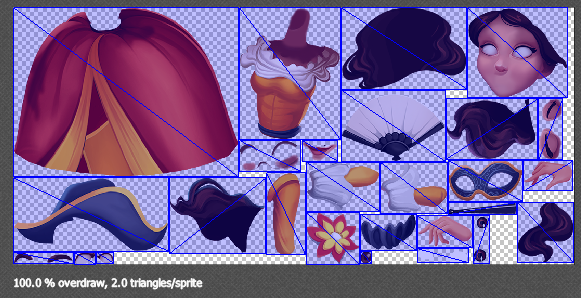
\includegraphics[width=.59\linewidth]{RectangularPacking.png}
            \end{subfigure}
            \vskip .5cm
            \begin{subfigure}[H]{\linewidth}
                \centering
                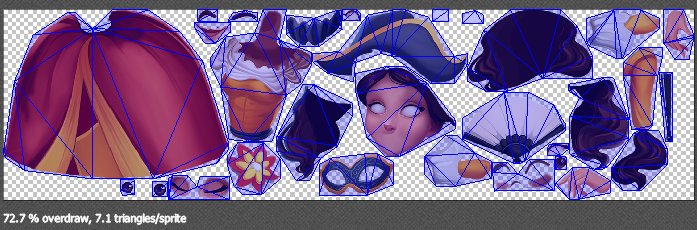
\includegraphics[width=.59\linewidth]{PolygonalPacking.png}
            \end{subfigure}
        \end{figure}
    \end{frame}
    \begin{frame}
        \frametitle{DistortionMesh}
        \begin{itemize}
            \item Структура меша -- регулярная сетка
            \item Вершина меша -- тяжеловесный объект.
        \end{itemize}
        \begin{figure}
            \centering
            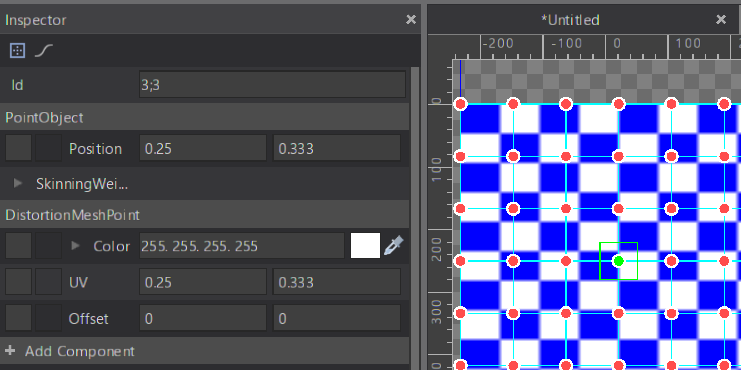
\includegraphics[scale=0.5]{DistortionMesh.png}
            \caption{DistortionMesh и DistortionMeshPoint -- объекты в иерархии сцены}
        \end{figure}
    \end{frame}
    \begin{frame}
        \frametitle{Цели и задачи}
        Цели:
        % \begin{itemize}

        % \end{itemize}
        Задачи:
        % \begin{itemize}

        % \end{itemize}
    \end{frame}
    \begin{frame}
        \frametitle{Этапы полигональной упаковки в атлас}
        \begin{itemize}
            \item Трассировка контура
            \item Генерация невыпуклой оболочки -- аппроксимация контура полигоном
            \item Генерация меша из невыпуклой оболочки
            \item Упаковка в атлас
        \end{itemize}
    \end{frame}
    \begin{frame}
        \frametitle{Трассировка контура}
    \end{frame}
    \begin{frame}
        \frametitle{Генерация невыпуклой оболочки}
    \end{frame}
    \begin{frame}
        \frametitle{Исследования генерации меша}
    \end{frame}
    \begin{frame}
        \frametitle{Триангуляция Делоне}
    \end{frame}
    \begin{frame}
        \frametitle{Добавление вершины, лежащей внутри триангуляции}
    \end{frame}
    \begin{frame}
        \frametitle{Добавление вершины, лежащей снаружи триангуляции}
    \end{frame}
    \begin{frame}
        \frametitle{Удаление вершины, лежащей внутри триангуляции}
    \end{frame}
    \begin{frame}
        \frametitle{Удаление граничной вершины}
    \end{frame}
    \begin{frame}
        \frametitle{Гипотеза перемещения}
    \end{frame}
    \begin{frame}
        \frametitle{Делоне с ограничениями}
    \end{frame}
    \begin{frame}
        \frametitle{PolygonMesh}
    \end{frame}
    \begin{frame}
        \frametitle{Полигональная упаковка}
    \end{frame}
    \begin{frame}
        \frametitle{Реализация}
    \end{frame}
    \begin{frame}
        \frametitle{Заключение}
    \end{frame}
\end{document}\frametitle{Триангуляция Делоне}
